\section{Surface Integrals}
\subsection{Parameterization of Surfaces}
Remember that early in the semester we dealt with parametric equations. Specifically, we dealt with \hyperlink{paraderiv}{parametric curves} in 3-dimensional space. However, we primarily dealt functions from $\bbr\to\bbr^3$, that is, functions with a single input that yielded a vector output, a 1-dimensional object in 3-dimensional space. However, we can also consider parametric surfaces, functions from $\bbr^2\to\bbr^3$, that yield 2-dimensional objects in 3-dimensional space. We briefly dealt with this topic when covering the \hyperlink{paraplane}{parametric form of a plane}.

\begin{definition}{Parametric Surface}
Let $\vcr(u,v)$ be a function from $\bbr^2\to\bbr^3$, where $$\vcr(u,v)=\bmat{x(u,v)\\y(u,v)\\z(u,v)}.$$ The outputs vector valued function as a set of points in $\bbr^3$ defines a parametric surface $S$ in $3$-dimensional space.
\end{definition}

Note that we can actually consider any of the \hyperlink{surf1}{surfaces} we looked at in the second part of this class as parametric surfaces.

\begin{example}{A Surface, Parameterized}
Let $f(x,y)=10-x^2+y^3-3y^2-6y$. Then we can parameterize this surface by letting $x(u,v)=u$, $y(u,v)=v$, and $z(u,v)=f(u,v)$. Then we get the parameterization $$\vcr(u,v)=\bmat{u\\v\\10-u^2+v^3-3v^2-6v}.$$
\end{example}

\begin{exercise}{Identifying and Parameterizing Surfaces}
\begin{enumerate}
\item Consider the parametric surface $$\vcr(\theta,\phi)=\bmat{4\sin(\phi)\cos(\theta)\\4\sin(\phi)\sin(\theta)\\4(\cos(\phi)}.$$ What does this surface represent? Hint: Consider the \hyperlink{spherical}{spherical transformation for triple integrals}.
\vspace{1em}
\item Parameterize a cylinder with radius of 3 where the cross sections parallel to the $xy$-plane are circles. (i.e. it's height runs parallel to the $z$ axis). Hint: Consider the \hyperlink{cylind}{cylindrical transformation for triple integrals}.
\end{enumerate}
\end{exercise}

We can also find planes tangent to parametric surfaces. We'll use partial derivatives, much like we did before, so let's state what the partial derivative of a parametric surface is.

\begin{definition}{Partial Derivative of a Parametric Surface}
Let $$\vcr(u,v)=\bmat{x(u,v)\\y(u,v)\\z(u,v)}$$ be a parametric surface where $x,y,z$ are differentiable functions. Then define the partial derivatives as \begin{align*}
\vcr_u(u,v)=&\bmat{\frac{\del}{\del u}\big(x(u,v)\big)\\\frac{\del}{\del u}\big(y(u,v)\big)\\\frac{\del}{\del u}\big(z(u,v)\big)}=\bmat{x_u(u,v)\\y_u(u,v)\\z_u(u,v)}\\
\vcr_v(u,v)=&\bmat{\frac{\del}{\del v}\big(x(u,v)\big)\\\frac{\del}{\del v}\big(y(u,v)\big)\\\frac{\del}{\del v}\big(z(u,v)\big)}=\bmat{x_v(u,v)\\y_v(u,v)\\z_v(u,v)}
\end{align*}
\end{definition}

Note that if we take some $\vcr(u,v)$ and some fixed point on the surface $(u_0,v_0)$, then $\vcr(u,v_0)$ and $\vcr(u_0,v)$ are both parametric curves that pass through the point $(u_0,v_0)$. Then $\vcr_u(u_0,v_0)$ gives a vector tangent to $\vcr(u,v_0)$ at $(u_0,v_0)$, and $\vcr_v(u_0,v_0)$ gives a vector tangent to $\vcr(u_0,v)$ at $(u_0,v_0)$. These two vectors should be independent from each other and parallel to the plane tangent to $\vcr(u,v)$ at $(u_0,v_0)$, so we can generate the equation of the plane by using the cross product of the two derivatives to find a normal vector!

\begin{example}{Tangent Plane}
Consider the parametric surface $S$, parameterized by $$\vcr(u,v)=\bmat{4\sin(u)\cos(v)\\4\sin(u)\sin(v)\\4\cos(u)}.$$ From before, we know this represents a sphere of radius 4, centered at the origin. Let's find the plane tangent to $S$ at $u=\frac{\pi}{6}$ and $v=\frac{\pi}{6}$. 
\vspace{1em}
\begin{center}
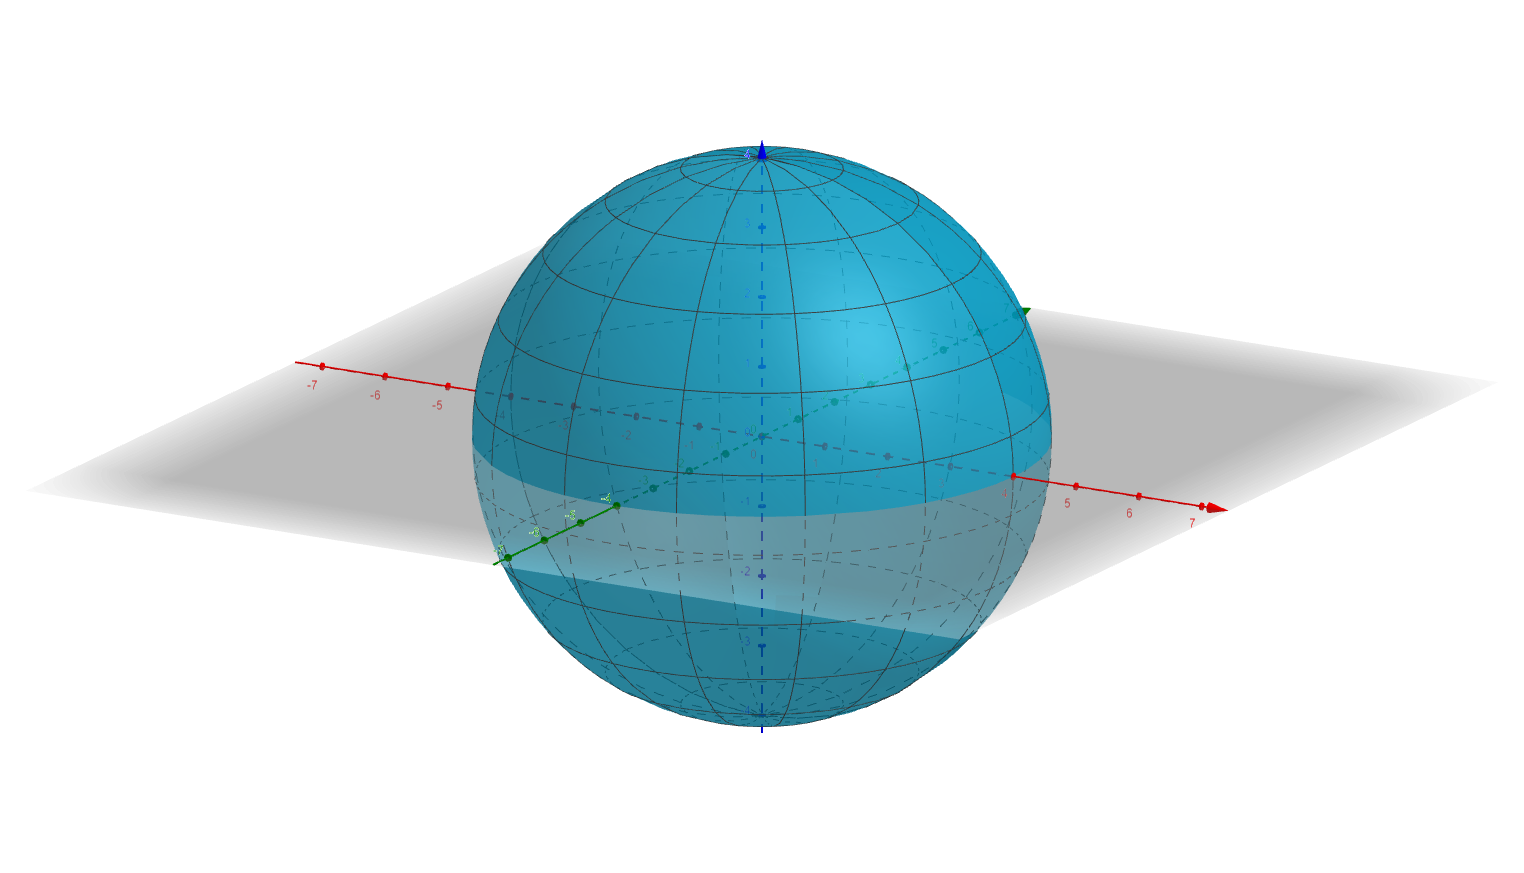
\includegraphics[scale=0.3]{Figures/sphere}\\
The surface $S$ (\href{https://www.geogebra.org/3d/hmgt3b7w}{Geogebra Link}).
\end{center}
\vspace{1em}
To find the tangent plane, we'll first need to find our two partial derivatives.
\begin{align*}
\vcr_u(u,v)=&\bmat{4\cos(u)\cos(v)\\4\cos(u)\sin(v)\\-4\sin(u)}\\
\vcr_v(u,v)=&\bmat{-4\sin(u)\sin(v)\\4\sin(u)\cos(v)\\0}\\
\end{align*}
Then we can plug in our values, which yields:
$$\vcr_u\left(\frac{\pi}{6},\frac{\pi}{6} \right)=\bmat{3\\ \sqrt{3}\\-2},\ \vcr_v\left(\frac{\pi}{6},\frac{\pi}{6} \right)=\bmat{-1\\ \sqrt{3}\\0}.$$
\begin{center}
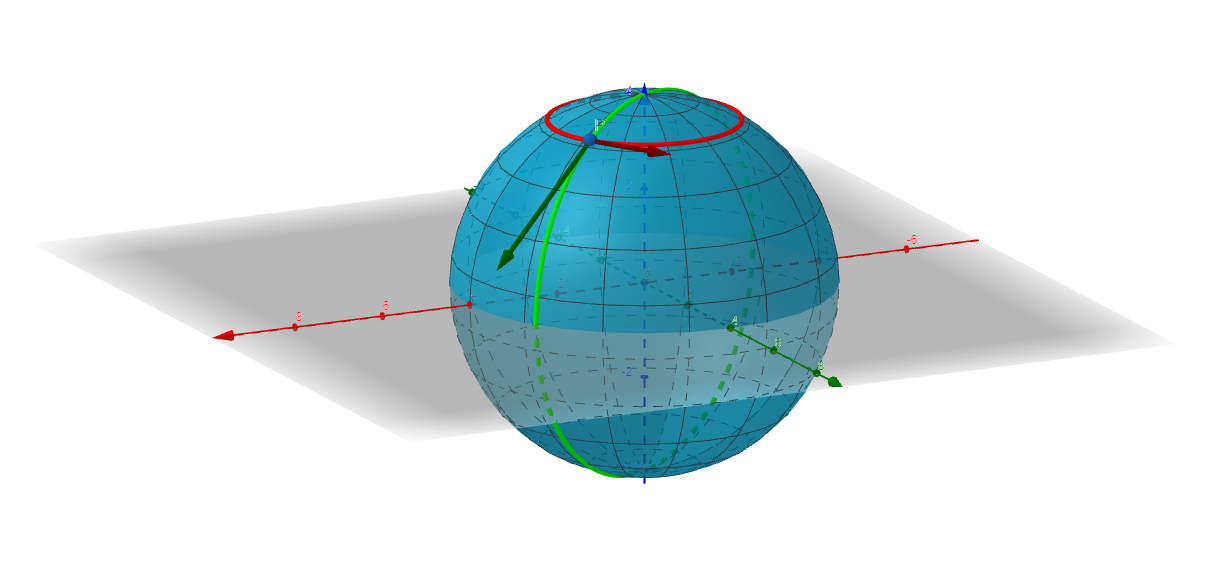
\includegraphics[scale=0.3]{Figures/surftan}\\
The surface $S$ with tangent vectors (\href{https://www.geogebra.org/3d/s78y49td}{Geogebra Link}).
\end{center}
\vspace{1em}
Then we can cross these two tangent vectors together to get the normal vector to our plane.
\begin{align*}\vcr_u\left(\frac{\pi}{6},\frac{\pi}{6} \right)\times\vcr_v\left(\frac{\pi}{6},\frac{\pi}{6} \right)=&\bmat{3\\ \sqrt{3}\\-2}\times\bmat{-1\\ \sqrt{3}\\0}\\
=&\det\bmat{\vci&\vcj&\vck\\3&\sqrt{3}&-2\\-1&\sqrt{3}&0}\\
=&\bmat{2\sqrt{3}\\2\\4\sqrt{3}}.
\end{align*}
Now we need only the coordinates of our point on the curve as $(x,y,z)$, which we find by evaluating $\vcr(u,v)$ at $u=\frac{\pi}{6}$ and $v=\frac{\pi}{6}$
$$\vcr\left(\frac{\pi}{6},\frac{\pi}{6} \right)=\bmat{\sqrt{3}\\1\\\ 2\sqrt{3}}. $$
Then we can use vector dot product form to generate the equation of our plane, then simplify to standard form.
\begin{align*}
2\sqrt{3}(x-\sqrt{3})+2(y-1)+4\sqrt{3}(z-2\sqrt{3})=&0\\
2\sqrt{3}x-6+2y-2+4\sqrt{3}z-24=&0\\
2\sqrt{3}x+2y+4\sqrt{3}z=&32\\
\sqrt{3}x+y+2\sqrt{3}z=&16.
\end{align*}\begin{center}
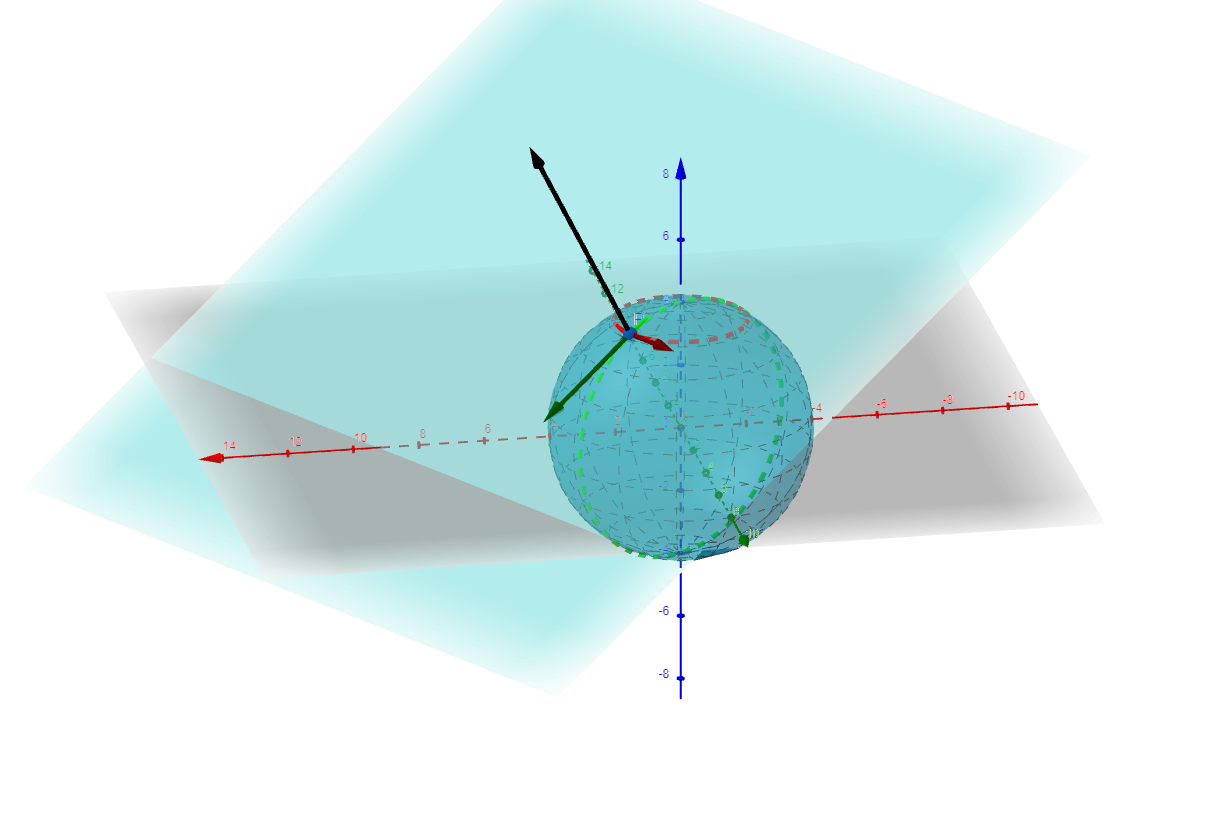
\includegraphics[scale=0.3]{Figures/surftan3}\\
The surface $S$ with tangent plane (\href{https://www.geogebra.org/3d/psngscyc}{Geogebra Link}).
\end{center}
\end{example}

\begin{exercise}{Is it a Bird? No, it's a Tangent Plane.}
\begin{enumerate}
\item Find the plane tangent to the \href{https://www.geogebra.org/3d/ympnc8vk}{surface $S$} parameterized by $$\vcr(u,v)=\bmat{u-4\\v^2\\u^2-2u+1}$$ at $u=2$, $v=1$.
\vspace{1em}
\item Find the plane tangent to the \href{https://www.geogebra.org/3d/dkmxdxkq}{surface $S$} parameterized by $$\vcr(u,v)=\bmat{v\\2\cos(u)\\2\sin(u)}$$ at $u=\frac{\pi}{4}$, $v=2$.
\end{enumerate}
\end{exercise}